\documentclass{article}
\usepackage{lmodern}

\usepackage{graphicx}
\graphicspath{{../figures/}} % Required for inserting images
\usepackage{tcolorbox}

\usepackage[ruled,vlined]{algorithm2e}
\usepackage{booktabs}
\usepackage{amsmath}
\usepackage{mathtools}
\usepackage{amssymb}
\usepackage{tabularx}
\usepackage{float}

\usepackage[round,authoryear]{natbib}
\usepackage{amsthm}

\newtheorem{definition}{Definition}
\newtheorem{proposition}{Proposition}
\newtheorem{theorem}{Theorem}
\newtheorem{lemma}{Lemma}
\newtheorem{remark}{Remark}
\newtheorem{corollary}{Corollary}

\usepackage[
    top=1in,
    bottom=1in,
    left=1in,
    right=1in,
    includehead,
    includefoot
]{geometry}

\usepackage[hidelinks]{hyperref} % keep last


\renewcommand{\algorithmautorefname}{Algorithm}


\title{Training-Free Ranking from Pairwise Comparisons via Acyclic Graph Construction}



\author{Soroush Vahidi\\
New Jersey Institute of Technology, Newark, NJ, USA\\
\texttt{sv96@njit.edu}\\
\href{https://orcid.org/0000-0003-1934-6282}{ORCID: 0000-0003-1934-6282}}




\date{}

\begin{document}



\maketitle

\begin{abstract}
Ranking from weighted pairwise comparisons asks for a global order that respects observed preferences as well as possible. We study a training-free, deterministic pipeline that builds an acyclic backbone on the comparison digraph using an MWFAS-inspired local-ratio heuristic, restores high-weight arcs under exact cycle-safe reinsertion, optionally applies a secondary weighted min-cut exchange, and extracts scores with optional order-preserving refinement. The local-ratio and exact add-back components follow prior lineage; this paper formalizes ranking--MWFAS optimum-value equivalence and practical guarantee boundaries, corrects a fixed-topological-position proxy weakening of add-back, and expands classical and GNN evaluation under timeout-aware common-completion analysis. Empirically, the canonical reachability-aware method (\textsc{OURS-Reach}) is strong on simple/naive upset metrics against several baselines, remains competitive rather than uniformly superior to SpringRank on family-aware checks, and is weaker than BTL on upset\_ratio. It is slower than most lightweight classical estimators yet substantially faster than archived trained GNNRank runs under an end-to-end protocol; the near-complete Finance graph marks a large-dense scalability boundary.
\end{abstract}
\newcommand{\keywords}[1]{\textbf{Keywords:} #1}

\keywords{Ranking; Pairwise comparisons; Feedback arc set; Directed graphs; Training-free methods}
\section{Introduction}
\label{sec:intro}
Ranking from pairwise comparisons arises throughout statistics, machine learning, and network analysis, from sports analytics to preference aggregation. Methods typically return a real-valued score vector whose induced order is evaluated by upset-based losses \citet{he22}. Classical estimators are fast and training-free; learning-based directed GNNs such as GNNRank can be accurate but introduce training cost, hyperparameter sensitivity, and reduced reproducibility.

Directed comparison graphs almost always contain cycles arising from noise, incompleteness, and local inconsistencies. A combinatorial response is to delete a set of directed arcs so that the remaining graph is acyclic, then read a ranking from a topological order of the resulting directed acyclic graph (DAG). This is the Minimum Weighted Feedback Arc Set (MWFAS) viewpoint: minimize the total weight of deleted comparisons subject to acyclicity. Related spectral and synchronization methods already note connections between ranking inconsistency and feedback structure \citet{SerialRank,SyncRank}. MWFAS is NP-hard \citet{K72}, so exact minimization is generally impractical, yet the formulation supplies a precise consistency-restoration objective for ranking.

This paper develops a practical, training-free, deterministic, and time-bounded ranking pipeline rather than a new general MWFAS approximation algorithm (\S\ref{sec:related}). Prior work by \citet{VK25} already used the local-ratio heuristic of Demetrescu and Finocchi \citet{CI03} with weight-prioritized exact cycle-safe reinsertion and optional refinement. We clarify that lineage, correct an implementation-fidelity gap, add theory and a secondary structural repair, and expand empirical validation.

To make the ranking--MWFAS connection precise, we begin with formal definitions.

\begin{definition}[Ranking Problem]
Let $G=(V,E)$ be a directed graph, where $V$ is the set of items and $E$ is the set of directed pairwise-comparison edges.
Each edge $(i,j)\in E$ has weight $w_{ij}>0$, representing the strength of the preference for $i$ over $j$.
A \emph{ranking} is a total order on $V$, represented equivalently by a bijection $R:V\rightarrow\{1,\dots,|V|\}$, where smaller values indicate higher rank.
An edge $(i,j)$ is \emph{inconsistent} with $R$ if $R(i)>R(j)$.
The goal is to find a ranking that minimizes the total weight of inconsistent edges:
\begin{equation}
\label{eq:ranking_obj}
\min_{R}\ \sum_{(i,j)\in E:\ R(i)>R(j)} w_{ij}.
\end{equation}
\end{definition}

\begin{definition}[Minimum Weighted Feedback Arc Set (MWFAS)]
Let $G=(V,E)$ be a directed graph with edge weights $w_{ij}>0$ for each $(i,j)\in E$.
A set of edges $F\subseteq E$ is a \emph{feedback arc set} if removing $F$ makes the graph acyclic, i.e., $(V,E\setminus F)$ is a directed acyclic graph (DAG).
The MWFAS problem is
\begin{equation}
\label{eq:mwfas}
\min_{F\subseteq E}\ \sum_{(i,j)\in F} w_{ij}
\quad \text{s.t.} \quad (V,E\setminus F)\ \text{is acyclic.}
\end{equation}
\end{definition}

The ranking objective~\eqref{eq:ranking_obj} and MWFAS~\eqref{eq:mwfas} share the same optimum \emph{value}: the backward edges of any ranking form a feedback arc set of equal weight, and any feedback arc set induces a DAG whose topological orders realize that deleted weight as ranking disagreement. The correspondence between optimal rankings and optimal feedback arc sets is many-to-many rather than one-to-one; we treat this equivalence as a formal claim to be stated and proved, not merely asserted.

\subsection{Scope, lineage, and contributions}
The pipeline studied here (\S\ref{sec:framework}) builds an acyclic backbone with the local-ratio heuristic of \citet{CI03}, reinserts high-weight arcs while preserving acyclicity, extracts scores from the resulting DAG, and optionally applies order-preserving refinement. Several components are \emph{prior}: local-ratio Phase~A, exact cycle-safe add-back (including weight ordering), and ternary/refinement ideas already appear in \citet{CI03,VK25}. What this paper contributes is therefore not a reinvention of that core, but the following.

\begin{enumerate}
\item \textbf{Formalization and guarantee boundaries.}
Ranking--MWFAS optimum-value equivalence (Prop.~\ref{prop:rank_mwfas}), implementation complexity, and when the Demetrescu--Finocchi guarantee does and does not transfer (\S\ref{subsec:theory_df03}).
\item \textbf{Implementation-fidelity correction.}
Restore exact reachability-aware reinsertion in place of a fixed-topological-position proxy (\S\ref{subsec:framework_phaseB}); ablations quantify the effect (\S\ref{subsec:ablation}).
\item \textbf{Secondary structural repair.}
A conflict-triggered weighted min-cut exchange with monotone objective improvement (Prop.~\ref{prop:mincut}), with regime-specific empirics (\S\ref{subsec:mincut_emp}).
\item \textbf{Expanded empirical validation.}
Classical and GNN comparisons with timeout-aware common completions, paired statistics, family-aware sensitivity, and ablation/sensitivity analysis (\S\ref{sec:exp}). Dataset-count expansion is not treated as a primary novelty.
\end{enumerate}

\subsection{Related Work}
\label{sec:related}

\subsubsection{Feedback Arc Set and MWFAS}
The Minimum Weighted Feedback Arc Set (MWFAS) problem asks for a minimum-weight set of directed arcs whose removal makes a graph acyclic \citet{K72,FPP20}. Classical approximation results include divide-and-conquer methods based on spreading metrics and LP relaxations \citet{EG95,EG2000}. Exact and parameterized algorithms target smaller or structurally restricted instances \citet{BA21,HM21,RS06,SJ21}. Heuristic refinements emphasize minimal/stable feedback sets and initialization effects \citet{c24,c25}. Closely related is the maximum acyclic subgraph problem \citet{HR94}. We use MWFAS as a ranking consistency objective, not as a setting in which we claim a new general approximation algorithm.

\subsubsection{Ranking from Pairwise Comparisons}
Ranking from noisy and incomplete pairwise comparisons has been studied through statistical, spectral, random-walk, and optimization-based formulations \citet{H00,CGZ21,SW16}. Our experiments evaluate score-based outputs under the upset-style losses used in recent ranking benchmarks \citet{he22}, so we focus on the principal baseline families represented in that protocol.

\subsubsection{Statistical and Spectral Ranking}
\textsc{BTL} models pairwise win probabilities through latent abilities \citet{BTL}. \textsc{DavidScore} aggregates unbalanced paired outcomes into per-item scores \citet{DavidScore}. Random-walk and spectral constructions include \textsc{RankCentrality} \citet{NS17}, \textsc{SerialRank} \citet{SerialRank}, \textsc{SyncRank} \citet{SyncRank}, and SVD-based scores \citet{SVD_RS_NRS}. Graph scoring methods include eigenvector centrality \citet{EigenvectorCentrality}, \textsc{PageRank} \citet{PageRank}, and \textsc{SpringRank} \citet{SpringRank}. Spectral and synchronization approaches already note connections between ranking inconsistency and feedback structure \citet{SerialRank,SyncRank}.

\subsubsection{GNN-Based Ranking}
Learning-based methods infer ranking scores from directed comparison graphs. \textsc{GNNRank} uses directed-GNN backbones with ranking-oriented losses \citet{he22}. We compare against the framework's \textsc{DIGRAC} \citet{DIGRAC} and inception-style (\textsc{ib}) \citet{DiGCN} backbones. These methods can be accurate but incur training cost and hyperparameter sensitivity, which motivates a training-free alternative under fixed wall-clock budgets.

\subsubsection{Local-Ratio Cycle Breaking, Add-Back Lineage, and Structural Repair}
Demetrescu and Finocchi \citet{CI03} give a local-ratio cycle-breaking heuristic with an approximation guarantee parameterized by the length of a longest simple directed cycle, building on the local-ratio framework of \citet{BK04}. Their Phase~2 reinserts deleted arcs subject to an \emph{exact} cycle-safety test (equivalently: reinsert $(u,v)$ iff $v$ does not reach $u$ in the current DAG), and they remark that ordering candidates by decreasing weight can improve solution quality. Exact cycle-safe reinsertion and weight-prioritized ordering are therefore prior; they are not newly invented here.

\subsubsection{Relation to \citet{VK25}}
\citet{VK25} operationalizes ranking via the \citet{CI03} local-ratio backbone with descending-weight exact cycle-safe reinsertion and order-preserving ternary refinement.
A later practical codebase weakened reinsertion to a fixed topological-position proxy; multipass INS variants partially compensate and are ablation baselines only.
Table~\ref{tab:novelty_separation} summarizes what is prior, restored for fidelity, or newly analyzed here.

\begin{table}[t]
\centering
\small
\setlength{\tabcolsep}{3.5pt}
\begin{tabular}{@{}lccc@{}}
\toprule
\textbf{Component} & \textbf{DF03} & \textbf{VK25} & \textbf{This work} \\
\midrule
Local-ratio backbone & yes & yes & prior (used) \\
Exact cycle-safe reinsertion & yes & yes (spec.) & fidelity restore \\
Weight-ordered reinsertion & suggested & yes & prior (used) \\
Time-bounded practical impl.\ & -- & partial & audited \\
Order-preserving refinement & -- & yes & prior (used) \\
Formal ranking$\leftrightarrow$MWFAS & -- & asserted & proved \\
DF03 guarantee under timeout & N/A & not audited & qualified (no) \\
Weighted min-cut exchange & -- & -- & secondary new \\
Broad classical + GNN eval.\ & -- & GNN-focused & expanded \\
\bottomrule
\end{tabular}
\caption{Novelty separation relative to Demetrescu--Finocchi (DF03) and \citet{VK25}. ``Fidelity restore'' means restoring the established exact test after an implementation weakening, not inventing the test.}
\label{tab:novelty_separation}
\end{table}

\section{Method and Theory}
\label{sec:framework}

We describe a deterministic, training-free ranking pipeline for weighted pairwise-comparison graphs. The canonical pipeline is:
\begin{enumerate}
\item \textbf{Phase~A (prior):} local-ratio-style cycle breaking \citet{CI03,VK25}.
\item \textbf{Phase~B (fidelity correction):} exact weight-prioritized reachability-aware reinsertion \citet{CI03,VK25}.
\item \textbf{Optional secondary repair (new):} conflict-triggered weighted min-cut exchange.
\item \textbf{Phase~C (prior lineage):} topological score extraction and optional order-preserving refinement \citet{VK25}.
\end{enumerate}
Fixed-topological-position multipass variants (INS1--3) are retained only as ablation contrasts (\S\ref{subsec:ablation}).

\subsection{Problem Setting}
\label{subsec:framework_problem}
Let $V=\{1,\dots,n\}$ be items and $G=(V,E,w)$ a directed graph with strictly positive arc weights $w:E\to\mathbb{R}_{>0}$. Antiparallel arcs are allowed. The solver input is a sparse weighted adjacency matrix converted to arrays $(\texttt{src},\texttt{dst},\texttt{w})$ of length $m=|E|$. The output is a score vector $s\in\mathbb{R}^n$ with larger values indicating higher rank. Formal ranking and MWFAS definitions appear in \S\ref{sec:intro}.

\subsection{Ranking--MWFAS Optimum-Value Equivalence}
\label{subsec:theory_equivalence}

\begin{proposition}[Optimum-value equivalence]
\label{prop:rank_mwfas}
Let $G=(V,E,w)$ with $w>0$. Write
\[
\mathrm{OPT}_{\mathrm{rank}}
=
\min_{R}\sum_{(i,j)\in E:\,R(i)>R(j)} w_{ij},
\qquad
\mathrm{OPT}_{\mathrm{MWFAS}}
=
\min\bigl\{\textstyle\sum_{e\in F}w_e : F\subseteq E,\ (V,E\setminus F)\ \text{acyclic}\bigr\}.
\]
Then $\mathrm{OPT}_{\mathrm{rank}}=\mathrm{OPT}_{\mathrm{MWFAS}}$.
The correspondence between optimal rankings and optimal feedback arc sets is many-to-many: we do \emph{not} claim a bijection between arbitrary rankings and arbitrary feedback arc sets.
\end{proposition}

\begin{proof}
Write $L(R)=\sum_{(i,j)\in E:\,R(i)>R(j)} w_{ij}$ for the ranking loss of $R$.

($\mathrm{OPT}_{\mathrm{MWFAS}}\le\mathrm{OPT}_{\mathrm{rank}}$.)
Fix any ranking $R$ and let $F_R=\{(i,j)\in E:R(i)>R(j)\}$. Every retained arc is forward under $R$, so $R$ is a topological order of $(V,E\setminus F_R)$ and $F_R$ is a feedback arc set of weight $L(R)$. Hence $\mathrm{OPT}_{\mathrm{MWFAS}}\le L(R)$ for every $R$, and taking the best ranking yields $\mathrm{OPT}_{\mathrm{MWFAS}}\le\mathrm{OPT}_{\mathrm{rank}}$.

($\mathrm{OPT}_{\mathrm{rank}}\le\mathrm{OPT}_{\mathrm{MWFAS}}$.)
Let $F^\star$ be an optimal feedback arc set and let $R$ be any topological order of the DAG $(V,E\setminus F^\star)$. Every retained arc is forward under $R$, so the set of backward arcs of $R$ is contained in $F^\star$. Therefore $L(R)\le w(F^\star)=\mathrm{OPT}_{\mathrm{MWFAS}}$, which implies $\mathrm{OPT}_{\mathrm{rank}}\le\mathrm{OPT}_{\mathrm{MWFAS}}$.
\end{proof}

\begin{remark}
If $F$ is inclusion-minimal, then for every topological order $R$ of $(V,E\setminus F)$ one has $L(R)=w(F)$. Optimal feedback arc sets under strictly positive weights are inclusion-minimal, but the optimum-value claim above does not require uniqueness of $F^\star$ or of $R$.
\end{remark}

\subsection{Unified Pipeline Pseudocode}
\label{subsec:pseudocode}

\begin{algorithm}[H]
\caption{Canonical ranking pipeline (training-free)}
\label{alg:ours_canonical}
\KwIn{Weighted digraph $G=(V,E,w)$; wall-clock budget $T$; zero tolerance $\tau$; optional min-cut flag; refinement budgets}
\KwOut{Score vector $s:V\to\mathbb{R}$}
$t_0\leftarrow\mathrm{now}()$;\ $r_e\leftarrow w_e$,\ $\mathrm{alive}_e\leftarrow\mathrm{true}$ for all $e\in E$\;
\While{$\mathrm{true}$}{
  \If{$\mathrm{now}()-t_0>T$}{\textbf{break}\tcp*{may exit while cyclic}}
  $C\leftarrow\mathrm{FindOneCycle}(\mathrm{alive})$ with deterministic vertex/edge order\;
  \If{$C=\emptyset$}{\textbf{break}\tcp*{acyclic}}
  $\Delta\leftarrow\min_{e\in C} r_e$\;
  \eIf{$\Delta\le 0$}{force-kill $\arg\min_{e\in C} r_e$}{
    $r_e\leftarrow r_e-\Delta$ for $e\in C$\;
    delete $\{e\in C:r_e\le\tau\}$;\ \If{none deleted}{force-kill $\arg\min_{e\in C} r_e$}
  }
}
$\mathrm{kept}\leftarrow\mathrm{alive}$\tcp*{Phase~A output}
sort excluded arcs by descending $w$, stable ties by edge id\;
\ForEach{excluded arc $e=(u,v)$ in that order}{
  \If{$\mathrm{now}()-t_0>T$}{\textbf{break}}
  \If{$v\not\rightarrow^\star u$ in current kept DAG}{$\mathrm{kept}[e]\leftarrow\mathrm{true}$}
}
\If{min-cut repair enabled}{apply Alg.~\ref{alg:mincut_exchange} under remaining budget}\;
$\pi\leftarrow\mathrm{TopoSort}(\mathrm{kept})$;\ \If{$\pi=\mathrm{None}$}{$\pi\leftarrow(1,\dots,n)$\tcp*{identity fallback}}
$s_v\leftarrow\max\{1,n-\mathrm{pos}_\pi(v)\}$\;
optionally apply order-preserving refinement under remaining budget\;
\Return{$s$}
\end{algorithm}

\subsection{Phase~A: Local-Ratio Cycle Breaking (Prior)}
\label{subsec:framework_phaseA}
Phase~A follows the local-ratio reduction of \citet{CI03}: maintain residuals, find a directed cycle by deterministic DFS (vertices in increasing index order; outgoing arcs in stored order), subtract the cycle's minimum residual, and delete arcs whose residual falls to at most $\tau$. Forced-progress safeguards kill one minimum-residual arc if floating-point reduction would otherwise stall. Phase~A stops when the alive subgraph is acyclic or when the wall-clock budget expires. Acyclicity is guaranteed only on the former exit.

\subsection{Phase~B: Exact Reachability-Aware Reinsertion (Fidelity Correction)}
\label{subsec:framework_phaseB}
After Phase~A, excluded arcs are scanned once in stable descending original weight. Arc $(u,v)$ is reinserted iff there is no directed path $v\rightarrow^\star u$ in the current kept DAG. This is the exact cycle-safety test of \citet{CI03,VK25}. A fixed-topological-position proxy (accept iff $\mathrm{pos}(u)<\mathrm{pos}(v)$ for one fixed topological order) is weaker and is retained only as an ablation baseline (INS multipass variants).

\begin{proposition}[Exact add-back correctness]
\label{prop:reachability_addback}
Assume the Phase~A kept graph is a DAG. Consider a single descending-weight scan that inserts $(u,v)$ iff $v\not\rightarrow^\star u$ in the current kept DAG.
\begin{enumerate}
\item \textbf{Acyclicity.} Every accepted insertion preserves acyclicity.
\item \textbf{Monotonicity.} Insertions only enlarge reachability.
\item \textbf{One-pass sufficiency.} An arc rejected when scanned cannot become admissible later in the same monotone scan.
\item \textbf{Single-edge inclusion minimality.} After a complete exact scan, no excluded arc can be restored individually without creating a cycle.
\end{enumerate}
This is inclusion-minimality under single-edge restoration, not a claim of globally minimum-weight FAS.
\end{proposition}

\begin{proof}
(1) If adding $(u,v)$ created a cycle, the remainder of that cycle would be a $v\rightarrow^\star u$ path in the previous DAG, contradicting the acceptance test.
(2) Adding arcs cannot destroy existing paths.
(3) Suppose $(u,v)$ is unsafe at its turn, so a path $v\rightarrow^\star u$ exists. Later insertions only add arcs, so that path persists and $(u,v)$ remains unsafe.
(4) Completeness of the scan means every excluded arc was rejected exactly because restoring it alone would close a cycle.
\end{proof}

\subsection{Optional Secondary Repair: Weighted Min-Cut Exchange}
\label{subsec:framework_mincut}
Some high-weight excluded arcs remain unsafe because $v$ reaches $u$. For such an arc $e=(u,v)$, let $C$ be a minimum-capacity directed $v\rightarrow u$ cut in the retained DAG (capacities $=$ kept-arc weights). The candidate exchange is
\[
D'=(D\setminus C)\cup\{e\}.
\]
Accept only if $w(C)+\mathrm{tol}<w(e)$.

\begin{algorithm}[H]
\caption{Conflict-triggered weighted min-cut exchange (optional)}
\label{alg:mincut_exchange}
\KwIn{Kept DAG $D$; excluded arcs; budgets on candidates/acceptances; tolerance $\mathrm{tol}$}
\ForEach{unsafe candidate $e=(u,v)$ under a fixed deterministic order}{
  $C\leftarrow$ directed min $v\rightarrow u$ cut in $D$\;
  \If{$w(C)+\mathrm{tol}<w(e)$}{
    $D\leftarrow(D\setminus C)\cup\{e\}$\tcp*{strict weighted-FAS improvement}
  }
}
\end{algorithm}

\begin{proposition}[Min-cut exchange]
\label{prop:mincut}
Whenever an exchange is accepted under the strict rule $w(C)+\mathrm{tol}<w(e)$:
\begin{enumerate}
\item $D'$ is acyclic;
\item the removed-FAS weight changes by $\Delta=w(C)-w(e)<0$;
\item repeated accepted exchanges terminate after finitely many steps.
\end{enumerate}
We claim no global optimality and no approximation ratio for this operator. The guarantee is structural improvement of the weighted feedback objective; ranking metrics need not improve monotonically.
\end{proposition}

\begin{proof}
(1) Removing $C$ destroys every $v\rightarrow u$ path, so adding $(u,v)$ cannot close a cycle.
(2) Relative to the previous feedback set, arcs in $C$ re-enter the feedback set and $e$ leaves it, giving $\Delta=w(C)-w(e)$; acceptance forces $\Delta<0$.
(3) There are finitely many subsets of $E$, and each acceptance strictly decreases a nonnegative objective bounded below by $0$.
\end{proof}

\subsection{Phase~C: Scores and Optional Refinement (Prior Lineage)}
\label{subsec:framework_phaseC}
From a kept DAG we compute a deterministic topological order (Kahn's algorithm with index-ordered initial queue) and assign $s_v=\max\{1,n-\mathrm{pos}(v)\}$. If the kept graph is still cyclic (e.g., Phase~A timeout), the implementation falls back to the identity order $(1,\dots,n)$; see \S\ref{subsec:theory_fallback}. Optional adjacent-swap refinement may change the order under a local budget. Optional order-preserving ternary refinement adjusts magnitudes without changing the induced order, following the refinement lineage in \citet{VK25}.

\subsection{Termination, Parameters, and Determinism}
\label{subsec:parameters}
\begin{table}[H]
\centering
\small
\begin{tabular}{@{}llp{6.6cm}@{}}
\toprule
\textbf{Parameter} & \textbf{Role} & \textbf{Notes} \\
\midrule
$T$ (\texttt{time\_limit\_sec}) & Global wall-clock budget & Shared by Phases~A--C; early exit may leave cycles \\
$\tau$ (\texttt{zero\_tol}) & Residual kill threshold & Default $10^{-15}$; numerical, not a modeling knob \\
DFS / Kahn order & Deterministic traversal & Vertices $1..n$; stable edge order \\
Add-back order & Descending $w$, stable ties & Exact reachability test (canonical) \\
Legacy $P\in\{1,2,3\}$ & Fixed-topological-position passes & INS1/2/3 ablation baselines; not canonical \\
Min-cut budgets & Optional repair caps & Secondary; regime-specific benefit \\
Refinement budgets & Phase~C time/passes & Order-preserving ternary from prior lineage \\
Identity fallback & Score extraction if cyclic & No nontrivial general error bound (\S\ref{subsec:theory_fallback}) \\
\bottomrule
\end{tabular}
\caption{Consolidated parameters and termination behavior.}
\label{tab:parameters}
\end{table}

\subsection{DF03 Approximation Guarantee: Idealized vs.\ Practical}
\label{subsec:theory_df03}
\paragraph{Idealized local-ratio Phase~A.}
If Phase~A is executed under the assumptions of the published Demetrescu--Finocchi local-ratio procedure and runs to the relevant completion condition (fully reduced acyclic residual), the published $\lambda$-approximation on removed weight applies to that idealized algorithm, where $\lambda$ is governed by longest-cycle length in the source analysis \citet{CI03}.

\paragraph{Practical implementation.}
The implemented pipeline additionally uses finite wall-clock termination, floating-point zero tolerance, forced-progress safeguards, and a fallback ranking when topological sort fails. Therefore the original theorem does \emph{not} automatically imply that every practical finite-budget output satisfies the same approximation guarantee.

\begin{remark}[No inherited guarantee under premature termination]
\label{rem:no_df03_timeout}
\textbf{We do not claim the DF03 approximation guarantee for prematurely terminated practical runs.}
In particular, a wall-clock cutoff inside Phase~A may leave the kept graph cyclic; subsequent identity-order fallback is outside the theorem's scope.
\end{remark}

\subsection{Fallback Ordering: Unbounded Multiplicative Gap}
\label{subsec:theory_fallback}

\begin{proposition}[No nontrivial multiplicative bound for identity fallback]
\label{prop:fallback}
For every $M>0$ there exists a weighted digraph $G$ with $\mathrm{OPT}_{\mathrm{rank}}>0$ such that if $R_{\mathrm{fb}}$ denotes the identity ranking $R_{\mathrm{fb}}(v)=v$, then
\[
\frac{L(R_{\mathrm{fb}})}{\mathrm{OPT}_{\mathrm{rank}}}>M.
\]
\end{proposition}

\begin{proof}
Fix $\varepsilon\in(0,1)$ and an integer $n\ge 3$ large enough that $\binom{n}{2}/\varepsilon>M$.
On vertex set $\{1,\dots,n\}$, include every arc $(j,i)$ with $j>i$ and weight $1$, and add the single arc $(1,2)$ with weight $\varepsilon$.
Under the identity ranking $R_{\mathrm{fb}}(v)=v$, every arc $(j,i)$ with $j>i$ is backward, so $L(R_{\mathrm{fb}})=\binom{n}{2}$.
Under the reverse ranking $R^\star(v)=n+1-v$, every unit-weight arc is forward and only $(1,2)$ is backward, so $L(R^\star)=\varepsilon$ and thus $\mathrm{OPT}_{\mathrm{rank}}\le\varepsilon$.
Hence $L(R_{\mathrm{fb}})/\mathrm{OPT}_{\mathrm{rank}}\ge\binom{n}{2}/\varepsilon>M$.
(The same instances show that additive regret $L(R_{\mathrm{fb}})-\mathrm{OPT}_{\mathrm{rank}}$ is likewise unbounded as $n$ grows with $\varepsilon$ fixed.)
\end{proof}

\subsection{Complexity}
\label{subsec:framework_complexity}
Let $n=|V|$ and $m=|E|$. For the audited Phase~A implementation, each cycle search scans the static adjacency of all original arcs (dead arcs are skipped but not compacted), costing $O(n+m)$ per iteration, and at most $m$ iterations occur before acyclicity in the unbudgeted case. Therefore the idealized full-completion Phase~A bound is
\[
O(mn+m^2),
\]
which is weaker than a textbook $O(nm)$ accounting that assumes compacted alive adjacency. A wall-clock budget caps completed iterations empirically; it is an execution policy, not an average-case complexity theorem.

Exact reachability add-back costs $O(m\log m)$ for sorting plus polynomial-in-$n$ dense incremental updates (or BFS queries in a sparse fallback). Optional min-cut repair adds budgeted directed min-cut computations. Phase~C is time-bounded and may use up to $O(n^2)$ pairwise structures for ratio refinement. Empirical timing is reported in \S\ref{subsec:runtime_coverage}--\ref{subsec:scalability}.

\section{Experimental Results}
\label{sec:exp}

\subsection{Experimental Protocol}
\label{subsec:exp_setup}

\paragraph{Dataset suite and denominators.}
We use an $80$-dataset manuscript benchmark suite aligned with recent ranking-from-comparisons evaluations \citep{he22}, spanning basketball/football temporal graphs, faculty hiring networks, animal and head-to-head competition graphs, one ERO-style instance, and the near-complete Finance graph ($n=1315$, $m\approx 1.73\times 10^{6}$, density $\approx 1$).
Two suite members lack loadable adjacency files in the archived release (\texttt{ERO/p5K5N350eta10styleuniform}, \texttt{Halo2BetaData/HeadToHead}), so analyses that require readable graphs use an effective denominator of $78$ loadable datasets ($80-2=78$).
The loadable Halo family member is \texttt{Halo2BetaData}; \texttt{Halo2BetaData/HeadToHead} is a distinct suite ID without a resolvable \texttt{adj.npz} under the repository loader.
An extra inventory entry \texttt{\_AUTO/Basketball\_temporal\_\_1985adj} is excluded from the manuscript suite (it is a duplicate adjacency variant of Basketball 1985 and would otherwise inflate a raw repository count to $81$).
We never mix denominators: pairwise quality/runtime tables use method-pair common completions (typically $n=77$ for OURS vs classical; $n=60$ for OURS vs GNN), coverage uses the $78$ loadable graphs, and family-aware macros exclude Finance from quality aggregates.
Table~\ref{tab:dataset_suite_summary} summarizes families; non-Finance ablation successes reach $n\le 602$.

\begin{table}[H]
\centering
\small
\setlength{\tabcolsep}{4pt}
\begin{tabular}{@{}lrrrr@{}}
\toprule
\textbf{Family} & \textbf{\#} & $n$ min--max & $m$ min--max \\
\midrule
Basketball (coarse+finer) & 60 & 282--351 & 2{,}904--7{,}650 \\
Football (coarse+finer) & 12 & 20--20 & 107--380 \\
Faculty (3) & 3 & 113--206 & 1{,}204--1{,}787 \\
Halo / head-to-head & 2 & 602--602 & 5{,}010--5{,}010 \\
Animal & 1 & 21 & 193 \\
ERO-style & 1 & (suite range) & (suite range) \\
Finance & 1 & 1{,}315 & 1{,}729{,}225 \\
\bottomrule
\end{tabular}
\caption{Manuscript $80$-suite families (intended counts). Two missing adjacency files reduce loadable graphs to $78$.}
\label{tab:dataset_suite_summary}
\end{table}

\paragraph{Methods.}
Baselines are ten classical methods (\textsc{SpringRank}, \textsc{SyncRank}, \textsc{SerialRank}, \textsc{BTL}, \textsc{DavidScore}, eigenvector/\textsc{PageRank}/\textsc{RankCentrality}, \textsc{SVD-RS}/\textsc{SVD-NRS}) and two GNNRank backbones (\textsc{DIGRAC}, \textsc{ib}) under fixed archived configurations (not post-hoc best-in-suite oracles).
The \emph{canonical} method reported in the principal quality/runtime tables is \textsc{OURS-Reach}: Phase~A + exact reachability-aware reinsertion + Phase~C refinement (\S\ref{sec:framework}), \emph{without} the optional min-cut exchange.
Optional min-cut remains a secondary structural operator evaluated in ablation/empirics (\S\ref{subsec:ablation}, \S\ref{subsec:mincut_emp}).
Archived \textsc{OURS-MFAS}/\textsc{INS3} labels correspond to duplicate fixed-topological-position configurations retained only as ablation contrasts.

\paragraph{Determinism, repetitions, and timing.}
Non-GNN methods are deterministic given fixed inputs and completed work: ranking outputs do not vary across the protocol's $10$ recorded trials except through wall-clock/timeout effects.
Those repetitions characterize runtime variability and timeout repeatability; they are \emph{not} independent ranking observations.
GNN methods are stochastic under training.
Non-GNN wall-clock budgets use $1800$\,s; GNN runs use $7200$\,s.
Archived GNN timings measure the end-to-end trained pipeline (construction + training + scoring), not inference-only latency; the exact archived GPU model ledger is unavailable, so hardware comparability is imperfect and GNN speedups are qualified accordingly.

\paragraph{Completion rules and statistics.}
Timeouts, missing data, and GNN not-applicable cases are reported separately; we do not impute NaNs as scores.
Primary comparisons use pairwise common completions.
We report win/tie/loss (W/T/L) counts with ties $|\Delta|\le 10^{-6}$, median paired $\Delta$ (\textsc{OURS-Reach} $-$ baseline; for upset metrics, negative favors \textsc{OURS-Reach}), and---where precomputed---Wilcoxon signed-rank $p$-values with Holm adjustment and bootstrap CIs.
Because many basketball seasons are temporally related, we add a family-aware sensitivity analysis (\S\ref{subsec:family_aware}).

\paragraph{Canonical numerical source.}
Principal Tables~\ref{tab:pairwise_quality_simple}--\ref{tab:runtime_wtl} use \textsc{OURS-Reach} under the GNNRank upset metrics of \citet{he22}, paired against the archived baseline leaderboard.
Structural ablation results document stage contributions and the fixed-topological-position versus reachability contrast (\S\ref{subsec:ablation}).

\subsection{Direct Ranking Quality on Common Completions}
\label{subsec:main_quality}

Table~\ref{tab:pairwise_quality_simple} and Table~\ref{tab:pairwise_quality_ratio}
summarize \textsc{OURS-Reach} against principal baselines on pairwise common completions.

\begin{table}[H]
\centering
\small
\setlength{\tabcolsep}{4pt}
\begin{tabular}{@{}lrrrr@{}}
\toprule
\textbf{Baseline} & $n$ & W/T/L & med~$\Delta$ & Holm $p$ \\
\midrule
SpringRank & 77 & 64/0/13 & $-0.157$ & $1.1\times 10^{-10}$ \\
DavidScore & 77 & 75/0/2 & $-0.180$ & $<10^{-11}$ \\
SVD\_NRS & 77 & 76/0/1 & $-0.165$ & $<10^{-11}$ \\
BTL & 77 & 76/0/1 & $-0.422$ & $<10^{-11}$ \\
PageRank & 77 & 76/0/1 & $-0.349$ & $<10^{-11}$ \\
SyncRank & 77 & 77/0/0 & $-1.008$ & $<10^{-11}$ \\
SerialRank & 77 & 77/0/0 & $-1.247$ & $<10^{-11}$ \\
RankCentrality & 77 & 77/0/0 & $-1.254$ & $<10^{-11}$ \\
DIGRAC & 60 & 60/0/0 & $-0.316$ & $4.9\times 10^{-11}$ \\
ib & 60 & 60/0/0 & $-0.620$ & $4.9\times 10^{-11}$ \\
\bottomrule
\end{tabular}
\caption{\texttt{upset\_simple} (lower better) on pairwise common completions for \textsc{OURS-Reach}.
$\Delta=$ \textsc{OURS-Reach} $-$ baseline (negative favors \textsc{OURS-Reach}). Holm $p$ within this table's primary family.}
\label{tab:pairwise_quality_simple}
\end{table}

\begin{table}[H]
\centering
\small
\setlength{\tabcolsep}{4pt}
\begin{tabular}{@{}lrrr l@{}}
\toprule
\textbf{Baseline} & $n$ & W/T/L & med~$\Delta$ & Note \\
\midrule
SpringRank & 77 & 42/0/35 & $-0.030$ & competitive \\
DavidScore & 77 & 74/0/3 & $-0.084$ & \\
SVD\_NRS & 77 & 72/0/5 & $-0.089$ & \\
BTL & 77 & 3/0/74 & $+0.081$ & BTL stronger \\
PageRank & 77 & 14/0/63 & $+0.029$ & PageRank stronger \\
SyncRank & 77 & 47/0/30 & $-0.210$ & \\
SerialRank & 77 & 47/0/30 & $-0.125$ & \\
RankCentrality & 77 & 77/0/0 & $-0.593$ & \\
DIGRAC & 60 & 30/0/30 & $-0.039$ & \\
ib & 60 & 30/0/30 & $-0.149$ & \\
\bottomrule
\end{tabular}
\caption{\texttt{upset\_ratio} (lower better) on the same common completions for \textsc{OURS-Reach}.
Oracle best-in-suite envelopes are not headline competitors.}
\label{tab:pairwise_quality_ratio}
\end{table}

On \texttt{upset\_simple}, \textsc{OURS-Reach} records large W/T/L margins and significant Holm-adjusted Wilcoxon advantages against all listed classical and GNN baselines in Table~\ref{tab:pairwise_quality_simple}.
On \texttt{upset\_naive}, the same directional pattern holds (e.g., $46/0/31$ vs SpringRank; $76/0/1$ vs BTL; $60/0/0$ vs \textsc{ib}).
On \texttt{upset\_ratio}, BTL remains clearly stronger ($3/0/74$) and PageRank also wins more often ($14/0/63$); SpringRank is competitive ($42/0/35$).
We do not claim universal dominance on any metric.

\subsection{Family-Aware Robustness}
\label{subsec:family_aware}

Basketball seasons dominate per-dataset $n$ ($\approx 60/77$).
Equal-family macros (seven included families; Finance excluded from quality macros) preserve \texttt{upset\_simple} advantages for \textsc{OURS-Reach} vs BTL/PageRank/DavidScore/SVD\_NRS on six of seven families.
The Halo family is the main SpringRank exception; leave-one-family-out of Basketball-coarse moves the equal-family mean near zero, so SpringRank comparisons remain family-sensitive even though the pairwise Holm test is significant.
The BTL \texttt{upset\_ratio} disadvantage persists under equal-family scrutiny.
Family-level $n$ is too small for heavy per-family significance testing; we treat family-aware results as sensitivity, not as a replacement for pairwise tests.

\subsection{Runtime and Coverage}
\label{subsec:runtime_coverage}

\begin{table}[H]
\centering
\footnotesize
\begin{tabular}{@{}lrrrr r@{}}
\toprule
\textbf{Baseline} & $n$ & OURS faster & ties & slower & median ratio (OURS/base) \\
\midrule
SyncRank & 77 & 48 & 0 & 29 & $0.80\times$ ($\sim 1.2\times$ faster) \\
SpringRank & 77 & 15 & 0 & 62 & $5.7\times$ \\
BTL & 77 & 19 & 0 & 58 & $7.9\times$ \\
RankCentrality & 77 & 0 & 0 & 77 & $17\times$ \\
SerialRank & 77 & 0 & 0 & 77 & $32\times$ \\
SVD\_NRS & 77 & 0 & 0 & 77 & $60\times$ \\
DavidScore & 77 & 0 & 0 & 77 & $108\times$ \\
PageRank & 77 & 0 & 0 & 77 & $170\times$ \\
DIGRAC & 60 & 60 & 0 & 0 & $0.022\times$ ($\sim 45\times$ faster) \\
ib & 60 & 60 & 0 & 0 & $0.027\times$ ($\sim 37\times$ faster) \\
\bottomrule
\end{tabular}
\caption{Paired runtime W/T/L on common completions for \textsc{OURS-Reach}.
\textsc{OURS-Reach} is slower than most lightweight classical methods (comparable to SyncRank) and faster than archived trained-GNN end-to-end runs.}
\label{tab:runtime_wtl}
\end{table}

Coverage on $78$ loadable datasets: \textsc{OURS-Reach} $77/78$ ($98.7\%$; Finance timeout); most classical methods $78/78$ ($100\%$); SyncRank $77/78$ (Finance timeout); DIGRAC/ib $61/78$ ($78.2\%$, primarily not-applicable rather than timeout).
A global $60$-dataset subset where all methods finish exists but is GNN-applicability biased; pairwise completion remains primary.
Figure~\ref{fig:runtime_vs_edges} shows empirical \textsc{OURS-Reach} runtimes versus $m$ for non-Finance graphs.

\begin{figure}[H]
\centering
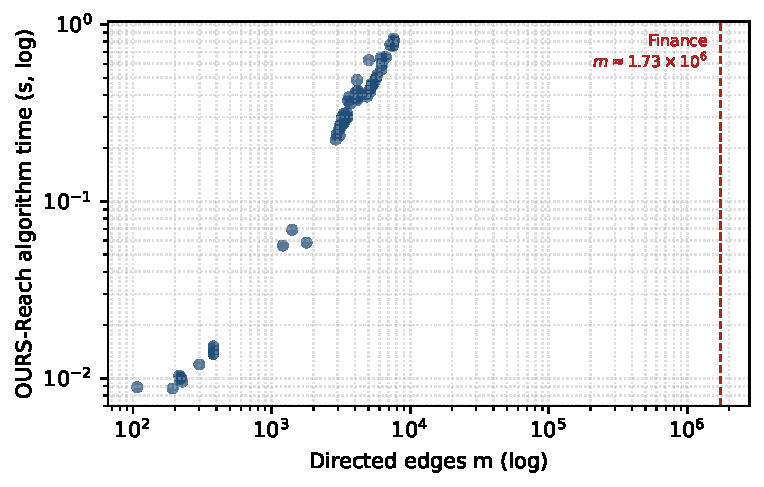
\includegraphics[width=0.72\linewidth]{fig_runtime_vs_edges.pdf}
\caption{\textsc{OURS-Reach} wall time versus edge count on non-Finance graphs (log--log). Finance ($m\approx 1.73\times 10^{6}$) is marked as the large-dense boundary.}
\label{fig:runtime_vs_edges}
\end{figure}

\subsection{Finance Stress Case}
\label{subsec:finance}

Finance is reported separately, not averaged into quality macros.
Under the archived $1800$\,s non-GNN protocol, fixed-topological-position OURS variants and SyncRank time out while lightweight classical methods finish in $<4$\,s and GNN end-to-end runs finish in $\sim 15$--$18$\,min.
Under a tightened Phase~A wall-clock budget of $600$\,s, Phase~A-only completes with wall $\approx 612.6$\,s (Phase~A $\approx 600.0$\,s); reachability and reachability+refinement configurations hit an internal time limit at $\approx 1214.8$/$1214.6$\,s; enabling optional min-cut hits a hard wall-clock timeout at $\approx 1800.1$\,s without a finished ranking.
This matches the $O(mn+m^{2})$ Phase~A discussion in \S\ref{subsec:framework_complexity}: Finance is a known large-dense boundary.

\subsection{Scalability (Empirical)}
\label{subsec:scalability}

On non-Finance ablation graphs ($n\le 602$), \textsc{OURS-Reach} finishes in roughly $0.01$--$1.2$\,s (median $\approx 0.57$\,s); enabling optional min-cut adds about $3$--$4$\,s median.
These timings illustrate the audited $O(mn+m^2)$ Phase~A bound (\S\ref{subsec:framework_complexity}) on sparse/moderate instances; the Finance boundary is in \S\ref{subsec:finance}. No fitted complexity law is claimed.

\subsection{Structural Ablation}
\label{subsec:ablation}

We use compact stage labels A0--A6:
A0~=~Phase~A only;
A1~=~fixed-topological-position add-back;
A2~=~exact reachability add-back;
A4~=~reachability+refinement (\textsc{OURS-Reach});
A5/A6~=~optional min-cut on top of A2/A4 (Layer-1 vs full).
Primary Holm family (exact CSV values):

\begin{table}[H]
\centering
\footnotesize
\begin{tabular}{@{}llrrrr@{}}
\toprule
\textbf{Pair} & \textbf{Metric} & $n$ & W/T/L & med~$\Delta$ & Holm $p$ \\
\midrule
A0$\to$A2 & upset\_simple$\downarrow$ & 77 & 76/0/1 & $-0.0166$ & $2.4\times 10^{-12}$ \\
A1$\to$A2 & upset\_simple$\downarrow$ & 33 & 32/0/1 & $-0.0159$ & $1.5\times 10^{-6}$ \\
A2$\to$A5 & removed weight$\downarrow$ & 33 & 26/7/0 & $-47$ & $8.3\times 10^{-6}$ \\
A4$\to$A6 & removed weight$\downarrow$ & 77 & 66/11/0 & $-57$ & $4.9\times 10^{-12}$ \\
A0$\to$A4 & upset\_simple$\downarrow$ & 77 & 76/0/1 & $-0.0169$ & $2.4\times 10^{-12}$ \\
\bottomrule
\end{tabular}
\caption{Primary structural ablation paired tests (non-Finance). Ranking metrics need not move monotonically with the weighted FAS objective (e.g., A4$\to$A6).}
\label{tab:ablation_primary}
\end{table}

Figure~\ref{fig:ablation} shows unpaired Layer median trajectories for context; paired tests above are authoritative.

\begin{figure}[H]
\centering
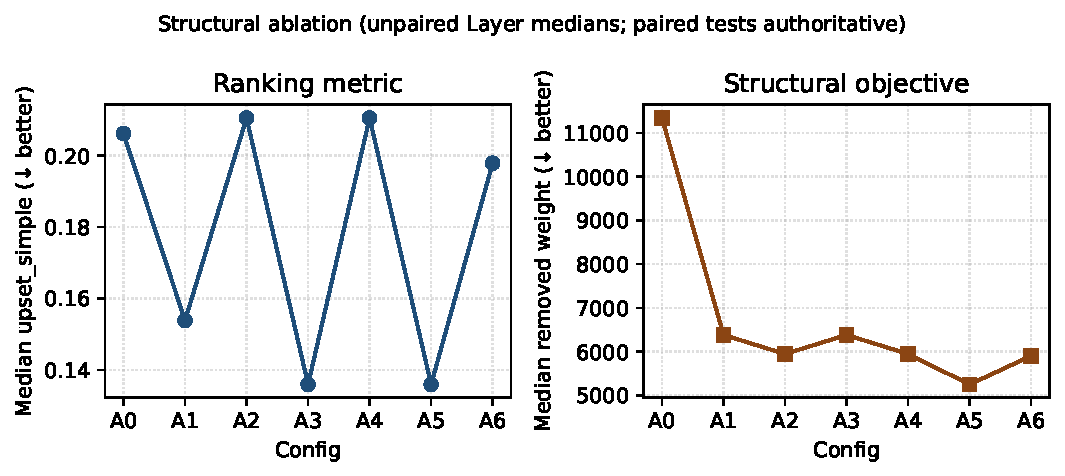
\includegraphics[width=0.95\linewidth]{fig_structural_ablation.pdf}
\caption{Unpaired median upset\_simple and removed weight across A0--A6 (descriptive).}
\label{fig:ablation}
\end{figure}

\subsection{Parameter Sensitivity (Compact)}
\label{subsec:sensitivity}

On Layer~1 ($n=33$): \texttt{zero\_tol} $\in\{10^{-12},10^{-15},10^{-18}\}$ is STABLE (almost all ties vs default).
Cycle-selection changes are statistically detectable on the reachability+refinement path but small ($|\mathrm{med}\,\Delta|\approx 10^{-3}$).
Refinement: R0 (off) is worse; R1$\approx$R2 and R3$\approx$R2 (saturation).
Fixed-topological multipass add-back: P1 restores many edges; P2/P3 add little ranking quality.
Min-cut budgets: K20$\to$K50 modest; K50$\to$K100 nearly flat. The main sensitivity trends relevant to the conclusions are summarized here.

\subsection{Min-Cut Empirical Regime}
\label{subsec:mincut_emp}
Under the predefined broad characterization (39 available of 40 datasets), the operator of \S\ref{subsec:framework_mincut} is active on $28/39$ graphs ($4/7$ families; $280$ accepted exchanges).
On active graphs, \texttt{upset\_simple}/\texttt{upset\_naive} never worsened; \texttt{upset\_ratio} worsened on $7/28$ (Basketball only; small magnitude), confirming regime-specific rather than universal ranking benefit.

\section{Limitations}
\label{sec:limitations}
Dense near-complete graphs remain difficult: Finance is the explicit boundary case documented in \S\ref{subsec:finance}.
Finite-budget practical outputs need not inherit the idealized Demetrescu--Finocchi guarantee (\S\ref{subsec:theory_df03}), and identity-order fallback has no nontrivial general multiplicative error bound (Prop.~\ref{prop:fallback}).
The optional min-cut repair improves the weighted feedback objective but not every upset metric, and its benefit is regime-specific (\S\ref{subsec:mincut_emp}).
Relative to most lightweight classical estimators \textsc{OURS-Reach} is slower (\S\ref{subsec:runtime_coverage}); GNN speedups refer to archived end-to-end training+evaluation under imperfect hardware comparability (\S\ref{subsec:exp_setup}).
Family-aware analysis shows that SpringRank comparisons remain family-sensitive, and BTL remains stronger on \texttt{upset\_ratio} (\S\ref{subsec:family_aware}).
Protocol repetitions for deterministic non-GNN methods characterize runtime/timeout variability rather than ranking uncertainty.

\section{Conclusion}
\label{sec:conclusion}
We addressed ranking from weighted pairwise comparisons with a training-free structural pipeline: local-ratio cycle breaking, exact reachability-aware reinsertion, optional weighted min-cut exchange, and score extraction/refinement.
The algorithmic core follows Demetrescu--Finocchi and \citet{VK25}; the contributions of this paper are formal ranking--MWFAS clarification and guarantee boundaries, restoration of exact cycle-safe add-back relative to a weaker fixed-topological-position rule, a secondary monotone min-cut repair, and a broader timeout-aware empirical study.

On common completions, \textsc{OURS-Reach} is strong on simple/naive upset metrics against the listed classical and GNN baselines, remains weaker than BTL on upset\_ratio, and is family-sensitive versus SpringRank despite a significant pairwise Holm test on upset\_simple.
It is slower than most lightweight classical methods (comparable to SyncRank), substantially faster than the evaluated trained GNN pipelines under the archived end-to-end protocol, and encounters a large-dense limit on Finance.

\section{Future Work}
\label{sec:future}
Theoretically, denser-graph cycle breaking, tighter analyses of time-bounded structural heuristics, and approximation results on restricted graph classes remain open.
Engineering directions include SCC-aware or parallel cycle processing, more efficient reachability maintenance, and better min-cut candidate selection under budgets.
Application settings such as preference aggregation, multi-source sensor comparisons, and industrial ranking are natural targets for the training-free pipeline but are not evaluated here.
Deterministic uncertainty quantification over multiple valid topological orders is another concrete direction.

\section*{Acknowledgments}
The author would like to express sincere gratitude to his family for their continued support and encouragement, and to Professor Ioannis Koutis for his guidance and support throughout this research. The author also thanks Anders Borum for generously providing complimentary lifetime access to Secure ShellFish, which supported the remote computing workflow used during this research.

\section*{Declaration of Generative AI and AI-assisted Technologies}
During the preparation and revision of this work, the author used ChatGPT (OpenAI), Claude (Anthropic), Cursor, and Perplexity AI to assist with manuscript organization and language refinement, literature and consistency checks, coding and analysis support, and preparation of responses to reviewer comments. All AI-assisted outputs, code, analyses, interpretations, citations, and manuscript changes were independently reviewed and verified by the author, who takes full responsibility for the scientific content and final manuscript.

\section*{Statements and Declarations}

\textbf{Funding}
The author received no financial support for the research, authorship, and/or publication of this article.

\textbf{Competing Interests}
The author declares that he has no competing interests.

\textbf{Ethics Approval}
Not applicable. This article does not report studies involving human participants or animals.

\textbf{Consent to Participate}
Not applicable.

\textbf{Consent for Publication}
Not applicable.

\textbf{Availability of Data and Materials}
The datasets used in the experiments originate from prior benchmarks cited in the manuscript (e.g., \cite{he22}). For reproducibility, the processed versions used in this study are provided as text files containing weighted directed edge lists in the public repository linked below.

\textbf{Code Availability}
All source code, processed data, and scripts required to reproduce the experiments are publicly available at \url{https://github.com/SoroushVahidi/ranking-by-feedback-arc-set}. The repository contains the implementation of the proposed method, the benchmark drivers, and the materials needed to reproduce the reported results. Implementations of the non-proposed baselines and the GNNRank training and evaluation pipeline are based on the public GNNRank codebase of \citet{he22}, with the corresponding adaptations documented in the repository.


\textbf{Author Contributions}
S. Vahidi is the sole author. He conceived the study, developed the algorithms, performed the experiments, and wrote the manuscript.



\bibliographystyle{apalike}  % Use 'apalike' instead of 'spbasic'
\bibliography{references}




\end{document}
